\chapter{Perancangan}
\label{perancangan} 

\section{Struktur Proyek Moodle Mobile}
\label{struktur proyek}

Proyek Moodle Mobile terdiri dari kumpulan file-file dan direktori-direktori utama yang mengandung fungsi dan \textit{source code} untuk aplikasi Moodle Mobile, platform Android dan iOS, alat untuk mebangun perangkat lunak, dan konfigurasi. Struktur proyek yang akan mengalami perubahan dapat dilihat pada Gambar \ref{moodle:projectstructure}.
\\
\begin{figure}[H]
%\dirtree{%
%.1 platforms/.
%.1 resources/.
%.1 node\_modules/.
%.1 src/.
%.2 app/.
%.2 config.json.
%.2 core/.
%.2 theme/.
%.1 config.xml.
%.1 ionic.config.json.
%}
\centering
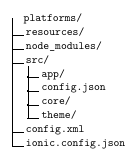
\includegraphics[scale = 1.5]{project-structure.PNG}
\caption{Struktur proyek moodleapp yang akan mengalami perubahan}
\label{moodle:projectstructure}
\end{figure}

Perubahan pada aplikasi akan sering dilakukan pada direktori \texttt{src}, dan \texttt{config.xml}. Direktori \texttt{src} berisi kode-kode utama dari aplikasi Moodle mobile dan konfigurasinya. Konfigurasi dari Moodle mobile sendiri diatur oleh file \texttt{config.json} di dalam folder \texttt{src}. File \texttt{Config.xml} berfungsi untuk mengatur konfigurasi dari aplikasi Cordova. Dikarenakan Moodle mobile menggunakan Cordova maka pengaturan saat melakukan \textit{build} untuk perangkat bergerak akan diambil dari file \texttt{config.xml}. 

Perubahan juga akan terjadi pada direktori \texttt{resources} dan file \texttt{ionic.config.json}. Direktori \texttt{resources} menyimpan sumber untuk ikon dan \textit{splashscreen} yang akan digunakan oleh aplikasi ketika di-\textit{build} untuk platform Android maupun iOS. File \texttt{ionic.config.json} adalah file konfigurasi yang digunakan oleh  Ionic CLI (\textit{Command Line Interface}), dimana nama aplikasi dan identifikasi aplikasi akan disimpan disana dan dirujuk oleh Ionic CLI ketika digunakan.

Direktori \texttt{node\_modules} juga akan mengalami perubahan namun jarang dilakukan perubahan secara langsung. Dikarenakan direktori tersebut menyimpan \textit{packages} yang dikelola oleh npm. Perubahan yang akan terjadi pada folder \texttt{node\_modules} adalah perubahan seperti yang dibahas di subbab \ref{moodle docs:env}.

\subsection{Perubahan pada \texttt{config.xml}}
Perubahan pada file \texttt{config.xml} akan berpengaruh ketika Cordova membangun aplikasi untuk Android dan iOS karena file \texttt{config.xml} mengatur aturan dan \textit{resource} apa saja yang akan digunakan oleh aplikasi di kedua platform tersebut. 

Perubahan yang dilakukan di dalam file ini adalah sebagai berikut : 

\begin{itemize}
\item Versi aplikasi untuk Android dan iOS akan dimulai dengan versi 1.0.0
\item Nama dari aplikasi adalah \textbf{IDE UNPAR Mobile}
\item Deskripsi aplikasi adalah \textbf{IDE UNPAR app}
\item Penulis aplikasi adalah \textbf{Gabriel Panji Lazuardi} dengan email \textbf{73160068@student.unpar.ac.id}
\item Ikon yang akan digunakan oleh aplikasi dalam platform Android dan iOS.
\item \textit{Splashscreen} yang akan digunakan aplikasi dalam platform Android dan iOS.
\end{itemize}  

\subsection{Perubahan pada direktori \texttt{src}}

Karena direktori ini mengandung \textit{source code} utama dari aplikasi, seluruh perubahan yang bersifat menambah, mengubah ataupun mengahpus fungsi di dalam aplikasi akan terjadi di dalam direktori \texttt{src}. Seluruh fungsi utama aplikasi terletak pada direktori \texttt{src/core}. Untuk pengaturan tema dari aplikasi terletak pada direktori \texttt{src/theme}. Dan folder \texttt{src/app} mengandung \textit{source code} yang akan dijalankan secara \textit{native} pada platform Android dan iOS seperti mengatur warna dari \textit{status bar}.	

Dalam folder \texttt{src/core} setiap fungsi dari Moodle mobile juga dipisah ke dalam direktori masing-masing. Setiap direktori dari fungsi-fungsi tersebut akan memiliki \textit{handler} dan \textit{helper}. Perubahan yang akan dilakukan pada file \textit{handler} adalah perubahan yang bersifat menerima dan memberi data dari dan untuk \textit{view}. Perubahan-perubahan pada \textit{helper} Moodle mobile akan bersifat untuk mengolah dan mengembalikan data.

\section{Menghubungkan IDE UNPAR Mobile dengan Situs IDE UNPAR}
\label{mobile:connect}
Menghubungkan IDE UNPAR mobile dengan situs IDE UNPAR dapat dilakukan dengan melakukan perubahan pada file \texttt{src/config.json}.  Perubahan yang harus dilakukan adalah menambahkan \textit{key} \textit{"siteurl"} dengan nilai URL yang diinginkan, dalam kasus ini URL yang akan digunakan adalah \url{https://ide.unpar.ac.id} dan mengkosongkan isi dari \textit{key "demo\_sites"}. Dengan adanya \textit{key "siteurl"} aplikasi saat dijalankan akan langsung melakukan koneksi dengan nilai dari \textit{key} tersebut. Sehingga ketika aplikasi IDE UNPAR mobile dijalankan, aplikasi akan langsung meminta pengguna \textit{login} dengan tautan \url{https://ide.unpar.ac.id}. 

\section{Penerapan Fitur-Fitur Tambahan dari Umpan Balik}
\label{feat:feedback}

Berdasarkan yang dibahas pada subbab \ref{feature feedback} beberapa saran fitur akan diimplementasikan pada aplikasi IDE UNPAR. Fitur-fitur tersebut adalah PDF \textit{scanner} dan .

\subsection{PDF \textit{scanner}}
\label{feat:pdfscan}
Fitur PDF \textit{scanner} tidak akan diimplementasikan selayaknya \textit{plugin} untuk Moodle mobile. Dikarenakan fitur ini hanya akan tersedia di dalam perangkat bergerak. Dan diperlukannya modifikasi pada file yang hanya berada di server IDE UNPAR. Implementasi fitur ini akan dilakukan dengan bantuan \textit{plugin} Cordova \texttt{cordova-pdf-generator} yang dibahas pada subbab \ref{pdf-gen}.
 
Implementasi fitur PDF \textit{scanner} ini akan dilakukan di direktori \texttt{src/core/fileuploader/}. Dimana \textit{handler} untuk fitur akan disimpan di \texttt{src/core/fileuploader/providers/scanner-handler.ts}. Untuk fungsi memindai gambar untuk diubah menjadi PDF sendiri akan disimpan di \\ \texttt{src/core/fileuploader/providers/helper.ts}. Dengan mengimplementasikan fitur ini pada direktori tersebut, maka fitur ini akan dapat digunakan untuk mengunggah file PDF ke dalam file pribadi pengguna di dalam server IDE UNPAR atau mengungghanya langsung sebagai bentuk submisi tugas atau quiz.\textit{Flow chart} untuk fitur dapat dilihat pada Gambar \ref{fig:scan:flowchart}. 

\begin{figure}[H] 
	\centering  
	\includegraphics[scale=0.6]{FlowChart-ScanPDF.png}  
	\caption[FlowChart untuk fitur PDF \textit{scanner}] {FlowChart untuk fitur PDF \textit{scanner}} 
	\label{fig:scan:flowchart} 
\end{figure} 

\subsection{Tautan menuju Student Portal UNPAR}
\label{feat:menu:link}
Seperti yang dibahas pada \ref{absesnsi IDE} akan diimplementasikan sebuah tautan pada menu aplikasi IDE UNPAR yang akan mengarahkan pengguna ke \url{https://studentportal.unpar.ac.id}. Selain menambahkan tautan, pilihan \texttt{change site} pada menu aplikasi akan dihapus karena dirasa pengguna tidak membutuhkan pilihan tersebut.

Perubahan yang harus dilakukan adalah menambahkan sebuah menu yang akan mengarahkan pengguna ke \url{https://sutdentportal.unpar.ac.id} pada \texttt{src/core/mainmenu\\/pages/more/more.html} ketika menu tersebut ditekan oleh pengguna. Dengan begitu pengguna dapat mengakses \url{https://studentportal.unpar.ac.id} melalui aplikasi IDE UNPAR mobile.

Perubahan selanjutnya yang harus dilakukan adalah menghapus pilihan \textit{change site} pada halaman menu aplikasi. Untuk menghapus pilihan tersebut dapat dilakukan dengan menghapus sebagian kode pada \texttt{src/core/mainmenu/pages/more/more.html}

\section{Meluncurkan Aplikasi ke dalam Google Play}
\label{apk:release}
Aplikasi akan diluncurkan ke dalam Goog Play yang dikelola oleh FTIS UNPAR. Untuk meluncurkan aplikasi ke dalam Google Play ada beberapa langkah yang harus dilakukan terlebih dahulu. Langkah-langkah tersebut akan dibahas di subsubbab-subsubbab berikut.

\subsection{Membuat apk \textit{release}}

Aplikasi IDE UNPAR Mobile harus dibangun terlebih dahulu dengan pengaturan \textit{production} dan \textit{release}. Membuat \textit{build} dengan pengaturan \textit{release} dapat dilakukan dengan menggunakan perintah \texttt{npx ionic cordova build android - -prod - -release}. Perintah tersebut akan menghasilkan sebuah apk di \texttt{/moodleapp/platforms/android/app/build/outputs/apk/release} dengan nama \texttt{app-release-unsigned.apk}. Namun, hanya dengan apk tersebut aplikasi tidak akan bisa dimasukkan ke dalam Google Play.

\subsection{Menandai aplikasi secara digital}
Google Play mengharuskan aplikasi yang akan diluncurkan untuk ditandai secara digital. Untuk melakukan hal tersebut diperlukannya sebuah \textit{keystore} yang dapat dibuat dengan \textit{keytool} yang disediakan oleh Java. Membuat \textit{keystore} dengan \textit{keytool} dapat dilakukan dengan perintah \texttt{keytool -genkey -v -keystore idemobile-release-key.keystore -alias ide-unpar-mobile -keyalg RSA \\ -keysize 2048 -validity 100000}, dengan menjalankan perintah tersebut maka sebuah file \textit{keystore} akan dihasilkan dengan nama \texttt{idemobile-release-key.keystore}.

Adanya file \textit{keystore} akan memungkinkan untuk menandai apk \textit{release} yang telah dibuat. Menandai apk dengan file \textit{keystore} dapat dilakukan dengan menggunakan jarsigner yang disediakan oleh Java. Menandai apk dengan jarsigner dilakukan dengan menjalankan perintah \texttt{jarsigner -verbose -sigalg SHA1withRSA -digestalg SHA1 -keystore idemobile-release-key.keystore \\ app-release-unsigned.apk ide-unpar-mobile}. 

\subsection{Finalisasi apk}
Optimasi yang dilakukan adalah menjalankan zipalign kepada apk yang telah ditandai secara digital. Karena pembanguna aplikasi tidak menggunakan Android Studio maka file apk harus di-zipalign secara manual. Zipalign dapat dijalankan dengan perintah \texttt{C:/Users/gabri/AppData/Local/Android/Sdk\\/build-tools/29.0.2/zipalign -v 4 app-release-unsigned.apk ideunparmobile.apk}. Perintah tersebut akan menghasilkan apk yang telah dikompresi dengan nama \texttt{ideunparmobile.apk}. Apk tersebut yang akan diunggah ke dalam Google Play.

\subsection{Mengunggah dan meluncurkan apk}
Apk dari aplikasi IDE UNPAR mobile akan diunggah dengan status \textit{open testing} ke dalam Google Play. Apk akan diunggah melalui Google Play Console. Untuk mengunggah aplikasi dengan status \textit{open testing}, pada menu Google Play Console pilih bagina \textit{Testing} dan kemudian \textit{Open Testing}. Ketika menu tersebut dipilih Google Play Console akan membukakan halaman \textit{Open Testing} seperti pada Gambar \ref{fig:play:open:test}. 

\begin{figure}[H] 
	\centering  
	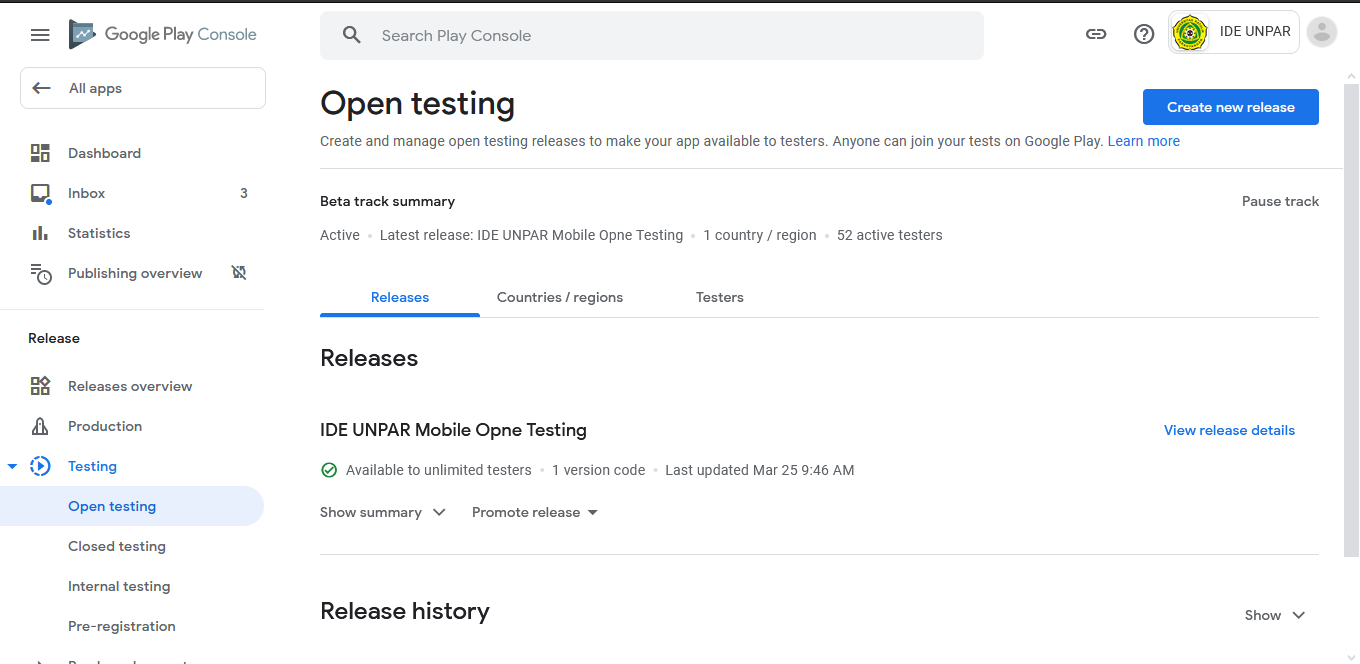
\includegraphics[scale=0.5]{play-console-menu.png}  
	\caption[Halaman \textit{Open Testing}] {Halaman \textit{Open Testing}} 
	\label{fig:play:open:test} 
\end{figure} 

Langkah selanjutnya adalah menekan tombol \textit{Create new release}. Menekan tombol tersebut akan membuka halaman \textit{Create open testing release} sepert pada Gambar \ref{fig:play:open:test:create}. Pada halaman tersebut apk akan diunggah dan detil dari \textit{release} akan diisi.  

\begin{figure}[H] 
	\centering  
	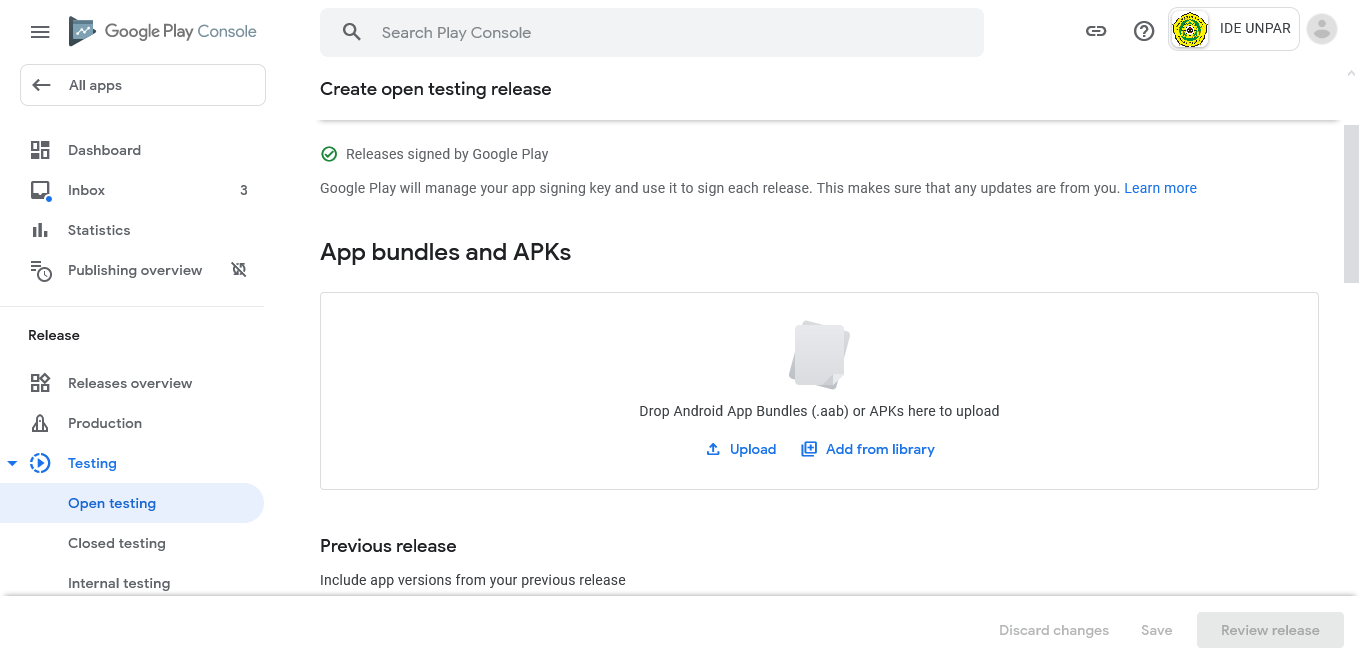
\includegraphics[scale=0.35]{play-create-open-test.png}  
	\caption[Halaman \textit{Create open testing release}] {Halaman \textit{Create open testing release}} 
	\label{fig:play:open:test:create} 
\end{figure} 

Sebelum dapat meluncurkan aplikasi ke dalam Google Play, \textit{release} yang baru saja dibuat harus simpan dan direview terlebih dahulu dengan menekan tombol \textit{Save} kemudian tombol \textit{Review release}. Menekan tombol \textit{Review release} akan membuka halam review seperti pada Gambar \ref{fig:play:open:test:review}. Apabila \textit{release} sudah direview \textit{release} dapat luncurkan dengan menekan tombol \textit{Start rollout to Open testing}.

\begin{figure}[H] 
	\centering  
	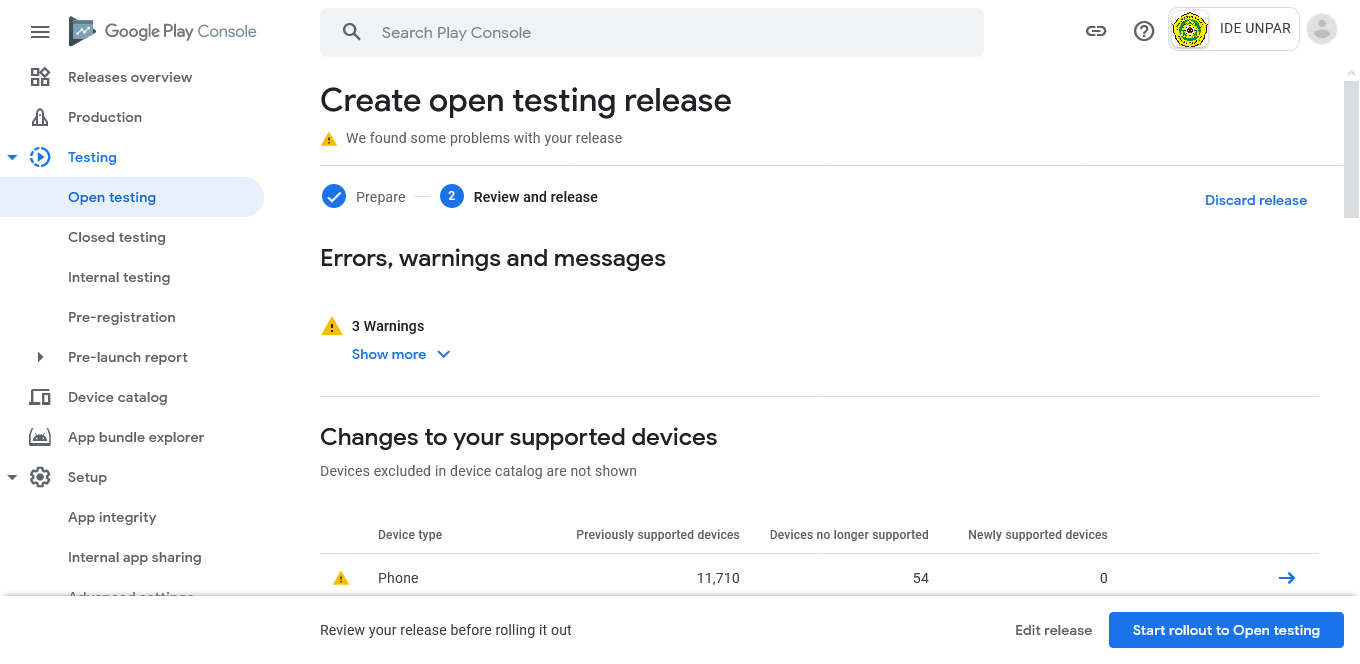
\includegraphics[scale=0.35]{play-review-release.png}  
	\caption[Halaman review \textit{Create open testing release}] {Halaman review \textit{Create open testing release}} 
	\label{fig:play:open:test:review} 
\end{figure} 